\chapter{Some Basic Notions of Set Theory}

\section{Ordered Pairs, Relations, and Functions}

\subsection*{Definitions and Theorems}

\begin{definition}[Ordered Pair]
The ordered pair $(a,b)$ is defined as the set $\{\{a\}, \{a,b\}\}$ (Kuratowski definition).
\end{definition}

\begin{theorem}[Equality of Ordered Pairs]
$(a,b) = (c,d)$ if and only if $a=c$ and $b=d$.
\end{theorem}

\begin{definition}[Relation]
A relation $R$ on a set $S$ is a subset of $S \times S$.
\end{definition}

\begin{definition}[Reflexive Relation]
A relation $R$ on $S$ is reflexive if $(x,x) \in R$ for all $x \in S$.
\end{definition}

\begin{definition}[Symmetric Relation]
A relation $R$ on $S$ is symmetric if $(x,y) \in R$ implies $(y,x) \in R$ for all $x,y \in S$.
\end{definition}

\begin{definition}[Transitive Relation]
A relation $R$ on $S$ is transitive if $(x,y) \in R$ and $(y,z) \in R$ implies $(x,z) \in R$ for all $x,y,z \in S$.
\end{definition}

\begin{definition}[Equivalence Relation]
A relation $R$ on $S$ is an equivalence relation if it is reflexive, symmetric, and transitive.
\end{definition}

\begin{definition}[Function]
A function $f: S \to T$ is a relation $f \subseteq S \times T$ such that for each $x \in S$, there exists exactly one $y \in T$ with $(x,y) \in f$.
\end{definition}

\begin{definition}[Domain and Codomain]
For a function $f: S \to T$, the set $S$ is called the domain and $T$ is called the codomain.
\end{definition}

\begin{definition}[Function Composition]
For functions $f: S \to T$ and $g: T \to U$, the composition $g \circ f: S \to U$ is defined by $(g \circ f)(x) = g(f(x))$.
\end{definition}

\begin{theorem}[Associativity of Function Composition]
If $f: S \to T$, $g: T \to U$, and $h: U \to V$ are functions, then $(h \circ g) \circ f = h \circ (g \circ f)$.
\end{theorem}



\begin{problembox}[2.1: Equality of Ordered Pairs]
Prove Theorem 2.2: $(a, b) = (c, d)$ if and only if $a=c$ and $b=d$.

Hint: $(a, b) = (c, d)$ means $\{\{a\}, \{a, b\}\} = \{\{c\}, \{c, d\}\}$. Now appeal to the definition of set equality.
\end{problembox}

\noindent\textbf{Strategy:} Use the Kuratowski definition of ordered pairs and set equality. Consider cases based on whether $a=b$ or $a\neq b$, then match elements of the sets to establish the required equalities.

\bigskip\noindent\textbf{Solution:}  
We must prove that $(a, b) = (c, d)$ if and only if $a=c$ and $b=d$.
The Kuratowski definition of an ordered pair is $(x, y) = \{\{x\}, \{x, y\}\}$.
If $a=c$ and $b=d$, then $(a,b) = \{\{a\}, \{a,b\}\} = \{\{c\}, \{c,d\}\} = (c,d)$. This direction is straightforward.

For the other direction, assume $(a, b) = (c, d)$. This means the sets are equal:
\[ \{\{a\}, \{a, b\}\} = \{\{c\}, \{c, d\}\} \]
By the definition of set equality, each element of the first set must be an element of the second, and vice versa. We consider two cases.

\textbf{Case 1: $a=b$.}
In this case, $(a, a) = \{\{a\}, \{a, a\}\} = \{\{a\}\}$.
For the sets to be equal, we must have $\{\{c\}, \{c, d\}\} = \{\{a\}\}$. This implies that the set $\{\{c\}, \{c, d\}\}$ has only one element, which means $\{c\} = \{c, d\}$. This equality holds if and only if $c=d$.
So we have $\{\{c\}\} = \{\{a\}\}$, which implies $\{c\} = \{a\}$, and thus $c=a$.
Since $c=d$ and $c=a$ and we started with $a=b$, we conclude that $a = b = c = d$. In particular, $a=c$ and $b=d$.

\textbf{Case 2: $a \neq b$.}
In this case, the set $\{\{a\}, \{a, b\}\}$ contains two distinct elements: the set $\{a\}$ with one member, and the set $\{a, b\}$ with two members. Therefore, the set $\{\{c\}, \{c, d\}\}$ must also contain two distinct elements, which implies $c \neq d$.
Since the sets are equal, their elements must match. We have two possibilities:
\begin{enumerate}
\item $\{a\} = \{c\}$ and $\{a, b\} = \{c, d\}$.
From $\{a\} = \{c\}$, we get $a=c$. Substituting this into the second equality gives $\{a, b\} = \{a, d\}$. Since $a \neq b$, the set on the left has two distinct elements. For the sets to be equal, we must have $b=d$. Thus, $a=c$ and $b=d$.
\item $\{a\} = \{c, d\}$ and $\{a, b\} = \{c\}$.
The first equality, $\{a\} = \{c, d\}$, would mean that the set $\{a\}$, which has one element, is equal to the set $\{c, d\}$, which has two elements (since $c \neq d$). This is impossible.
\end{enumerate}
The only possibility is that $a=c$ and $b=d$. In both cases, the equality of ordered pairs implies the equality of their corresponding components.\qed



\begin{problembox}[2.2: Properties of Relations]
Determine which of the following relations $S$ on $\mathbb{R}^2$ are reflexive, symmetric, and transitive:
\begin{enumerate}[label=(\alph*)]
\item $S = \{(x,y) \in \mathbb{R}^2 : x \leq y\}$
\item $S = \{(x,y) \in \mathbb{R}^2 : x < y\}$
\item $S = \{(x,y) \in \mathbb{R}^2 : x > y\}$
\item $S = \{(x,y) \in \mathbb{R}^2 : x^2 + y^2 \geq 1\}$
\item $S = \{(x,y) \in \mathbb{R}^2 : x^2 + y^2 < 0\}$
\item $S = \{(x,y) \in \mathbb{R}^2 : x^2 + x \leq y^2 + y\}$
\end{enumerate}
\end{problembox}

\noindent\textbf{Strategy:} Check each property systematically by testing specific values or finding counterexamples. For reflexivity, test $(x,x)$ pairs. For symmetry, check if $(x,y) \in S$ implies $(y,x) \in S$. For transitivity, verify if $(x,y), (y,z) \in S$ implies $(x,z) \in S$.

% Visualization for relation (d): x^2 + y^2 >= 1
\begin{figure}[h]
\centering
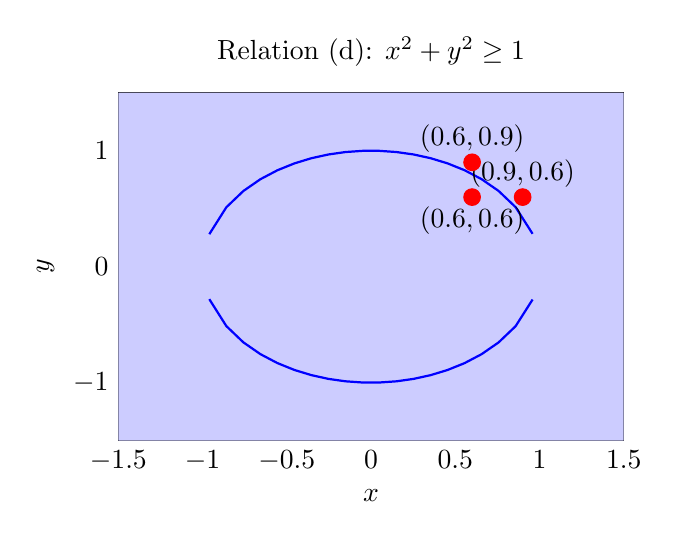
\begin{tikzpicture}
\begin{axis}[
    width=8cm,
    height=6cm,
    xlabel={$x$},
    ylabel={$y$},
    title={Relation (d): $x^2 + y^2 \geq 1$},
    xmin=-1.5, xmax=1.5,
    ymin=-1.5, ymax=1.5,
    grid=major,
    grid style={gray!30},
    samples=100
]

% Shaded region for x^2 + y^2 >= 1
\addplot[fill=blue!20, draw=none] {sqrt(1-x^2)};
\addplot[fill=blue!20, draw=none] {-sqrt(1-x^2)};
\addplot[fill=blue!20, draw=none] coordinates {(-1.5,-1.5) (-1.5,1.5) (1.5,1.5) (1.5,-1.5) (-1.5,-1.5)};

% Circle boundary
\addplot[blue, thick] {sqrt(1-x^2)};
\addplot[blue, thick] {-sqrt(1-x^2)};

% Counterexample points for transitivity
\addplot[red, mark=*, mark size=3pt] coordinates {(0.6,0.9)};
\node[above] at (axis cs:0.6,0.9) {$(0.6, 0.9)$};
\addplot[red, mark=*, mark size=3pt] coordinates {(0.9,0.6)};
\node[above] at (axis cs:0.9,0.6) {$(0.9, 0.6)$};
\addplot[red, mark=*, mark size=3pt] coordinates {(0.6,0.6)};
\node[below] at (axis cs:0.6,0.6) {$(0.6, 0.6)$};

\end{axis}
\end{tikzpicture}
\caption{The relation $x^2 + y^2 \geq 1$ is symmetric but not transitive. Points $(0.6,0.9)$ and $(0.9,0.6)$ are in the relation, but $(0.6,0.6)$ is not, providing a counterexample for transitivity.}
\end{figure}

\bigskip\noindent\textbf{Solution:}  
\begin{enumerate}[label=(\alph*)]
\item \textbf{Reflexive:} Yes - for all $x \in \mathbb{R}$, we have $x \leq x$ \\
\textbf{Symmetric:} No - if $x \leq y$ and $x \neq y$, then $y \not\leq x$ \\
\textbf{Transitive:} Yes - if $x \leq y$ and $y \leq z$, then $x \leq z$

\item \textbf{Reflexive:} No - $x < x$ is never true \\
\textbf{Symmetric:} No - if $x < y$, then $y \not< x$ \\
\textbf{Transitive:} Yes - if $x < y$ and $y < z$, then $x < z$

\item \textbf{Reflexive:} No - $x > x$ is never true \\
\textbf{Symmetric:} No - if $x > y$, then $y \not> x$ \\
\textbf{Transitive:} Yes - if $x > y$ and $y > z$, then $x > z$

\item  \textbf{Reflexive:}] No - the condition $(x,x) \in S$ requires $2x^2 \geq 1$, which fails for any $x$ in the interval $(-\frac{1}{\sqrt{2}}, \frac{1}{\sqrt{2}})$. \\
\textbf{Symmetric:} Yes - if $x^2 + y^2 \geq 1$, then $y^2 + x^2 \geq 1$ due to the commutative property of addition. 
\textbf{Transitive:} No - a counterexample is needed. Let $x = 0.6$, $y = 0.9$, and $z = 0.6$.
\begin{itemize}
\item $(x,y) \in S$ because $(0.6)^2 + (0.9)^2 = 0.36 + 0.81 = 1.17 \geq 1$.
\item $(y,z) \in S$ because $(0.9)^2 + (0.6)^2 = 0.81 + 0.36 = 1.17 \geq 1$.
\end{itemize}
However, $(x,z) \notin S$ because $(0.6)^2 + (0.6)^2 = 0.36 + 0.36 = 0.72 < 1$.

\item \textbf{Reflexive:} No - $x^2 + x^2 = 2x^2 \geq 0$ for all $x \in \mathbb{R}$ \\
\textbf{Symmetric:} Yes - if $x^2 + y^2 < 0$, then $y^2 + x^2 < 0$ \\
\textbf{Transitive:} Vacuously true - the relation is empty

\item \textbf{Reflexive:} Yes - for all $x \in \mathbb{R}$, $x^2 + x \leq x^2 + x$ \\
\textbf{Symmetric:} No - if $x^2 + x \leq y^2 + y$ and $x \neq y$, then $y^2 + y \not\leq x^2 + x$ \\
\textbf{Transitive:} Yes - if $x^2 + x \leq y^2 + y$ and $y^2 + y \leq z^2 + z$, then $x^2 + x \leq z^2 + z$
\end{enumerate}\qed



\begin{problembox}[2.3: Composition and Inversion of Functions]
The following functions \( F \) and \( G \) are defined for all real \( x \) by the equations given below. 

\textbf{Part 1.} In each case where the composite function \( G \circ F \) can be formed, give the domain of \( G \circ F \) and a formula (or formulas) for \( (G \circ F)(x) \):
\begin{itemize}
\item[(a)] \( F(x) = 1 - x \), \quad \( G(x) = x^2 + 2x \)
\item[(b)] \( F(x) = x + 5 \), \quad \( G(x) = \frac{|x|}{x} \), \( G(0) = 1 \)
\item[(c)] \( F(x) = \begin{cases} 2x, & 0 \le x \le 1 \\ 1, & \text{otherwise} \end{cases} \),  
\( G(x) = \begin{cases} 3x^2, & 0 \le x \le 1 \\ 5, & \text{otherwise} \end{cases} \)
\end{itemize}
\textbf{Part 2.} In the following, find \( F(x) \) if \( G(x) \) and \( G[F(x)] \) are given:
\begin{itemize}
\item[(d)] \( G(x) = x^3 \), \quad \( G[F(x)] = x^3 - 3x^2 + 3x - 1 \)
\item[(e)] \( G(x) = 3 + x + x^2 \), \quad \( G[F(x)] = x^2 - 3x + 5 \)
\end{itemize}
\end{problembox}

\noindent\textbf{Strategy:} For Part 1, substitute $F(x)$ into $G$ and simplify. For piecewise functions, determine which piece of $G$ applies based on the range of $F$. For Part 2, solve for $F(x)$ by recognizing patterns (like perfect cubes) or using algebraic manipulation.

% Visualization for piecewise functions in part (c)
\begin{figure}[h]
\centering
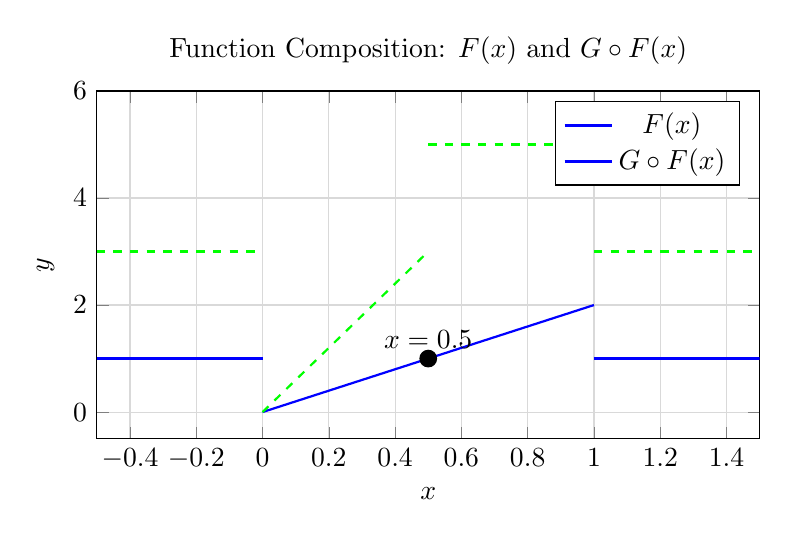
\begin{tikzpicture}
\begin{axis}[
    width=10cm,
    height=6cm,
    xlabel={$x$},
    ylabel={$y$},
    title={Function Composition: $F(x)$ and $G \circ F(x)$},
    xmin=-0.5, xmax=1.5,
    ymin=-0.5, ymax=6,
    grid=major,
    grid style={gray!30},
    legend pos=north east
]

% Function F(x)
\addplot[blue, thick] coordinates {(-0.5,1) (0,1)};
\addplot[blue, thick] coordinates {(0,0) (1,2)};
\addplot[blue, thick] coordinates {(1,1) (1.5,1)};
\addlegendentry{$F(x)$}

% Composition G o F
\addplot[green, thick, dashed] coordinates {(-0.5,3) (0,3)};
\addplot[green, thick, dashed] coordinates {(0,0) (0.5,3)};
\addplot[green, thick, dashed] coordinates {(0.5,5) (1,5)};
\addplot[green, thick, dashed] coordinates {(1,3) (1.5,3)};
\addlegendentry{$G \circ F(x)$}

% Mark key point
\addplot[black, mark=*, mark size=3pt] coordinates {(0.5,1)};
\node[above] at (axis cs:0.5,1) {$x=0.5$};

\end{axis}
\end{tikzpicture}
\caption{The piecewise functions $F(x)$ and their composition $G \circ F(x)$. The composition changes behavior at $x=0.5$ where $F(x)$ crosses from $[0,1]$ to $(1,2]$, causing the composition to switch from the quadratic rule to the constant rule.}
\end{figure}

\bigskip\noindent\textbf{Solution:}

\textbf{(a)}
The domain of both \(F\) and \(G\) is \(\mathbb{R}\), so the domain of \(G \circ F\) is \(\mathbb{R}\).
\begin{align*}
(G \circ F)(x) &= G(F(x)) \\
&= G(1-x) \\
&= (1-x)^2 + 2(1-x) \\
&= (1 - 2x + x^2) + (2 - 2x) \\
&= x^2 - 4x + 3
\end{align*}

\textbf{(b)}
The domain of \(F\) is \(\mathbb{R}\) and the domain of \(G\) is \(\mathbb{R}\), so the domain of \(G \circ F\) is \(\mathbb{R}\).
\begin{align*}
(G \circ F)(x) = G(F(x)) = G(x+5)
\end{align*}
We evaluate this based on the value of the input to \(G\), which is \(x+5\):
\[ (G \circ F)(x) = 
\begin{cases} 
\frac{|x+5|}{x+5} = 1, & \text{if } x+5 > 0 \implies x > -5 \\
1, & \text{if } x+5 = 0 \implies x = -5 \\
\frac{|x+5|}{x+5} = -1, & \text{if } x+5 < 0 \implies x < -5 
\end{cases}
\]
This simplifies to:
\[ (G \circ F)(x) = \begin{cases} -1, & x < -5 \\ 1, & x \ge -5 \end{cases} \]

\textbf{(c)}
The domain of \(G \circ F\) is \(\mathbb{R}\). We analyze the composition in pieces based on the definition of \(F(x)\).
\begin{itemize}
\item If $0 \le x \le 1$, then $F(x) = 2x$. The value of $F(x)$ is in the interval $[0, 2]$. We must check where $F(x)$ falls in the domain of $G$.
\begin{itemize}
\item If $0 \le F(x) \le 1$, which means $0 \le 2x \le 1$, or $0 \le x \le 0.5$. In this case, $G(F(x)) = 3(F(x))^2 = 3(2x)^2 = 12x^2$.
\item If $F(x) > 1$, which means $2x > 1$, or $0.5 < x \le 1$. In this case, $G(F(x)) = 5$.
\end{itemize}
\item If $x < 0$ or $x > 1$, then $F(x)=1$. Since this value is in the interval $[0,1]$, we use the first rule for $G$: $G(F(x)) = G(1) = 3(1)^2 = 3$.
\end{itemize}
Combining these results, we get the piecewise formula:
\[ (G \circ F)(x) = \begin{cases} 
3, & x < 0 \\
12x^2, & 0 \le x \le 0.5 \\
5, & 0.5 < x \le 1 \\
3, & x > 1
\end{cases}
\]

\textbf{(d)}
We are given $G(x) = x^3$ and $G[F(x)] = x^3 - 3x^2 + 3x - 1$.
The composition is $(F(x))^3$. We can recognize the expression for $G[F(x)]$ as the expansion of a cube:
\[ x^3 - 3x^2 + 3x - 1 = (x-1)^3 \]
Therefore, we have $(F(x))^3 = (x-1)^3$, which implies $F(x) = x-1$.

\textbf{(e)}
We are given $G(x) = 3 + x + x^2$ and $G[F(x)] = x^2 - 3x + 5$.
We set up the equation for the composition:
\begin{align*}
G(F(x)) &= 3 + F(x) + (F(x))^2 \\
x^2 - 3x + 5 &= 3 + F(x) + (F(x))^2
\end{align*}
Rearranging gives a quadratic equation in terms of $F(x)$:
\[ (F(x))^2 + F(x) + (3 - (x^2 - 3x + 5)) = 0 \]
\[ (F(x))^2 + F(x) + (-x^2 + 3x - 2) = 0 \]
We use the quadratic formula to solve for $F(x)$:
\begin{align*}
F(x) &= \frac{-1 \pm \sqrt{1^2 - 4(1)(-x^2+3x-2)}}{2(1)} \\
&= \frac{-1 \pm \sqrt{1 + 4x^2 - 12x + 8}}{2} \\
&= \frac{-1 \pm \sqrt{4x^2 - 12x + 9}}{2}
\end{align*}
The term under the square root is a perfect square: $4x^2 - 12x + 9 = (2x-3)^2$.
\[ F(x) = \frac{-1 \pm \sqrt{(2x-3)^2}}{2} = \frac{-1 \pm (2x-3)}{2} \]
This yields two possible functions for $F(x)$:
\begin{enumerate}
\item $F_1(x) = \frac{-1 + (2x-3)}{2} = \frac{2x-4}{2} = x-2$
\item $F_2(x) = \frac{-1 - (2x-3)}{2} = \frac{-2x+2}{2} = 1-x$
\end{enumerate}\qed



\begin{problembox}[2.4: Associativity of Function Composition]
Given three functions \( F, G, H \), what restrictions must be placed on their domains so that the following four composite functions can be defined?
\[
G \circ F, \quad H \circ G, \quad H \circ (G \circ F), \quad (H \circ G) \circ F
\]
Assuming that \( H \circ (G \circ F) \) and \( (H \circ G) \circ F \) can be defined, prove the associative law:
\[
H \circ (G \circ F) = (H \circ G) \circ F
\]
\end{problembox}

\noindent\textbf{Strategy:} For domain restrictions, ensure the range of each function is contained in the domain of the next function in the composition chain. For associativity, use the definition of function composition and show both sides evaluate to the same result.

\bigskip\noindent\textbf{Solution:}  
To define \( G \circ F \), the range of \( F \) must be contained in the domain of \( G \).  
To define \( H \circ G \), the range of \( G \) must be contained in the domain of \( H \).  
Under these conditions,  
\[
(H \circ (G \circ F))(x) = H(G(F(x))) = ((H \circ G) \circ F)(x)
\]  
So function composition is associative wherever defined.\qed

\section{Set Operations, Images, and Injectivity}

\subsection*{Definitions and Theorems}

\begin{definition}[Union]
The union of sets $A$ and $B$ is $A \cup B = \{x : x \in A \text{ or } x \in B\}$.
\end{definition}

\begin{definition}[Intersection]
The intersection of sets $A$ and $B$ is $A \cap B = \{x : x \in A \text{ and } x \in B\}$.
\end{definition}

\begin{definition}[Set Difference]
The difference of sets $A$ and $B$ is $A - B = \{x : x \in A \text{ and } x \notin B\}$.
\end{definition}

\begin{definition}[Complement]
The complement of a set $A$ with respect to a universal set $U$ is $A' = U - A$.
\end{definition}

\begin{definition}[Subset]
A set $A$ is a subset of a set $B$, written $A \subseteq B$, if every element of $A$ is also an element of $B$.
\end{definition}

\begin{definition}[Power Set]
The power set of a set $S$, denoted $\mathcal{P}(S)$, is the set of all subsets of $S$.
\end{definition}

\begin{theorem}[Set-Theoretic Identities]
For any sets $A$, $B$, and $C$:
\begin{enumerate}
\item $A \cup (B \cup C) = (A \cup B) \cup C$ (associativity of union)
\item $A \cap (B \cap C) = (A \cap B) \cap C$ (associativity of intersection)
\item $A \cap (B \cup C) = (A \cap B) \cup (A \cap C)$ (distributivity)
\item $A \cup (B \cap C) = (A \cup B) \cap (A \cup C)$ (distributivity)
\item $A \cap (B - C) = (A \cap B) - (A \cap C)$
\item $(A - C) \cap (B - C) = (A \cap B) - C$
\item $(A - B) \cup B = A$ if and only if $B \subseteq A$
\end{enumerate}
\end{theorem}

\begin{theorem}[Subset Transitivity]
If $A \subseteq B$ and $B \subseteq C$, then $A \subseteq C$.
\end{theorem}

\begin{definition}[Image]
For a function $f: S \to T$ and a subset $A \subseteq S$, the image of $A$ under $f$ is $f(A) = \{f(x) : x \in A\}$.
\end{definition}

\begin{definition}[Inverse Image]
For a function $f: S \to T$ and a subset $Y \subseteq T$, the inverse image of $Y$ under $f$ is $f^{-1}(Y) = \{x \in S : f(x) \in Y\}$.
\end{definition}

\begin{definition}[Injective Function]
A function $f: S \to T$ is injective (one-to-one) if $f(x_1) = f(x_2)$ implies $x_1 = x_2$ for all $x_1, x_2 \in S$.
\end{definition}

\begin{definition}[Surjective Function]
A function $f: S \to T$ is surjective (onto) if for every $y \in T$, there exists $x \in S$ such that $f(x) = y$.
\end{definition}

\begin{definition}[Bijective Function]
A function $f: S \to T$ is bijective if it is both injective and surjective.
\end{definition}

\begin{theorem}[Image of Unions and Intersections]
For a function $f: S \to T$ and subsets $A, B \subseteq S$:
\begin{enumerate}
\item $f(A \cup B) = f(A) \cup f(B)$
\item $f(A \cap B) \subseteq f(A) \cap f(B)$
\end{enumerate}
\end{theorem}

\begin{theorem}[Inverse Image Laws]
For a function $f: S \to T$ and subsets $Y_1, Y_2 \subseteq T$:
\begin{enumerate}
\item $f^{-1}(Y_1 \cup Y_2) = f^{-1}(Y_1) \cup f^{-1}(Y_2)$
\item $f^{-1}(Y_1 \cap Y_2) = f^{-1}(Y_1) \cap f^{-1}(Y_2)$
\item $f^{-1}(T - Y) = S - f^{-1}(Y)$
\end{enumerate}
\end{theorem}

\begin{theorem}[Image of Preimage and Surjectivity]
For a function $f: S \to T$, $f[f^{-1}(Y)] = Y$ for every $Y \subseteq T$ if and only if $f$ is surjective.
\end{theorem}

\begin{theorem}[Equivalent Conditions for Injectivity]
For a function $f: S \to T$, the following are equivalent:
\begin{enumerate}
\item $f$ is injective
\item $f(A \cap B) = f(A) \cap f(B)$ for all $A, B \subseteq S$
\item $f^{-1}[f(A)] = A$ for all $A \subseteq S$
\item For disjoint sets $A, B \subseteq S$, $f(A) \cap f(B) = \emptyset$
\item If $B \subseteq A$, then $f(A - B) = f(A) - f(B)$
\end{enumerate}
\end{theorem}



\begin{problembox}[2.5: Set-Theoretic Identities]
Prove the following set-theoretic identities:
\begin{itemize}
\item[(a)] \( A \cup (B \cup C) = (A \cup B) \cup C \), \quad \( A \cap (B \cap C) = (A \cap B) \cap C \)
\item[(b)] \( A \cap (B \cup C) = (A \cap B) \cup (A \cap C) \)
\item[(c)] \( (A \cap B) \cup (A \cap C) = A \cap (B \cup C) \)
\item[(d)] \( (A \cup B)(B \cup C)(C \cup A) = (A \cap B) \cup (A \cap C) \cup (B \cap C) \)
\item[(e)] \( A \cap (B - C) = (A \cap B) - (A \cap C) \)
\item[(f)] \( (A - C) \cap (B - C) = (A \cap B) - C \)
\item[(g)] \( (A - B) \cup B = A \) if and only if \( B \subseteq A \)
\end{itemize}
\end{problembox}

\noindent\textbf{Strategy:} Use element-chasing method: assume an element belongs to one side and show it belongs to the other side, then reverse the argument. For each identity, use the definitions of union, intersection, and set difference.

% Set operations Venn diagram
\begin{figure}[h]
\centering
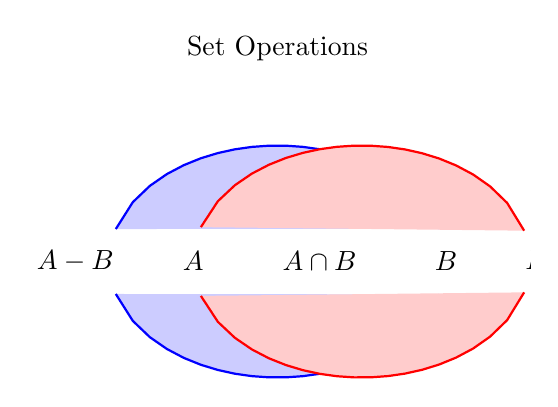
\begin{tikzpicture}
\begin{axis}[
    width=8cm,
    height=6cm,
    xlabel={},
    ylabel={},
    title={Set Operations},
    xmin=-1.5, xmax=1.5,
    ymin=-1.5, ymax=1.5,
    axis lines=none,
    samples=100
]

% Draw circles for sets A and B
\addplot[fill=blue!20, draw=blue, thick] {sqrt(1-x^2)};
\addplot[fill=blue!20, draw=blue, thick] {-sqrt(1-x^2)};
\addplot[fill=red!20, draw=red, thick] {sqrt(1-(x-0.5)^2)};
\addplot[fill=red!20, draw=red, thick] {-sqrt(1-(x-0.5)^2)};

% Add labels
\node at (axis cs:-0.5,0) {$A$};
\node at (axis cs:1,0) {$B$};
\node at (axis cs:0.25,0) {$A \cap B$};
\node at (axis cs:-1.2,0) {$A - B$};
\node at (axis cs:1.7,0) {$B - A$};

\end{axis}
\end{tikzpicture}
\caption{Venn diagram showing set operations. The union $A \cup B$ can be written as the disjoint union $A \cup (B - A)$, and the intersection $A \cap B$ shows the common elements.}
\end{figure}

\bigskip\noindent\textbf{Solution:}  
Each identity can be proven by element-chasing: assuming \( x \in \) one side and showing \( x \in \) the other side.  
For example, for (b), if \( x \in A \cap (B \cup C) \), then \( x \in A \) and \( x \in B \cup C \Rightarrow x \in (A \cap B) \cup (A \cap C) \). Similar for the reverse.\qed



\begin{problembox}[2.6: Image of Unions and Intersections]
Let \( f: S \to T \) be a function. If \( A \) and \( B \subseteq S \), prove:
\[
f(A \cup B) = f(A) \cup f(B), \quad f(A \cap B) \subseteq f(A) \cap f(B)
\]
Generalize to arbitrary unions and intersections.
\end{problembox}

\noindent\textbf{Strategy:} Use the definition of image of a set under a function. For unions, show that any element in the image of the union comes from either $A$ or $B$. For intersections, note that the inclusion may be strict due to non-injectivity.

\noindent\bigskip\noindent\textbf{Solution:}  
For any \( x \in A \cup B \), \( f(x) \in f(A) \cup f(B) \).  
For intersections, \( x \in A \cap B \Rightarrow f(x) \in f(A) \cap f(B) \), but the converse need not hold.  
Generalization:  
\[
f\left( \bigcup_i A_i \right) = \bigcup_i f(A_i), \quad f\left( \bigcap_i A_i \right) \subseteq \bigcap_i f(A_i)
\]\qed



\begin{problembox}[2.7: Inverse Image Laws]
Let \( f: S \to T \), and for any \( Y \subseteq T \), define the inverse image:
\[
f^{-1}(Y) = \{x \in S \mid f(x) \in Y \}
\]
Prove:
\begin{itemize}
\item[(a)] \( f^{-1}(Y_1 \cup Y_2) = f^{-1}(Y_1) \cup f^{-1}(Y_2) \)
\item[(b)] \( f^{-1}(T - Y) = S - f^{-1}(Y) \)
\end{itemize}
Generalize to arbitrary unions and intersections.
\end{problembox}

\noindent\textbf{Strategy:} Use the definition of inverse image and logical equivalence. For (a), show that $f(x) \in Y_1 \cup Y_2$ if and only if $f(x) \in Y_1$ or $f(x) \in Y_2$. For (b), use the fact that $f(x) \notin Y$ if and only if $x \notin f^{-1}(Y)$.

\noindent\bigskip\noindent\textbf{Solution:}  
(a) If \( x \in f^{-1}(Y_1 \cup Y_2) \), then \( f(x) \in Y_1 \cup Y_2 \Rightarrow x \in f^{-1}(Y_1) \cup f^{-1}(Y_2) \), and vice versa.  
(b) \( f(x) \notin Y \iff x \notin f^{-1}(Y) \Rightarrow x \in S - f^{-1}(Y) \)\qed



\begin{problembox}[2.8: Image of Preimage and Surjectivity]
Prove that \( f[f^{-1}(Y)] = Y \) for every \( Y \subseteq T \) if and only if \( f \) is surjective.
\end{problembox}

\noindent\textbf{Strategy:} For the forward direction, assume surjectivity and show that every element in $Y$ has a preimage in $f^{-1}(Y)$. For the reverse direction, assume the equality holds and show that if $f$ were not surjective, there would exist a $y \in T$ not in the image of any preimage.

\noindent\bigskip\noindent\textbf{Solution:}  
If \( f \) is surjective, every \( y \in Y \) has a preimage in \( S \), so is included in \( f[f^{-1}(Y)] \).  
If \( f \) is not surjective, then some \( y \notin f(S) \), and so not in the image of any preimage — thus excluded from \( f[f^{-1}(Y)] \).\qed



\begin{problembox}[2.9: Equivalent Conditions for Injectivity]
Let \( f: S \to T \) be a function. Show the following are equivalent:
\begin{itemize}
\item[(a)] \( f \) is injective
\item[(b)] \( f(A \cap B) = f(A) \cap f(B) \) for all \( A, B \subseteq S \)
\item[(c)] \( f^{-1}[f(A)] = A \) for all \( A \subseteq S \)
\item[(d)] For disjoint sets \( A, B \subseteq S \), \( f(A) \cap f(B) = \emptyset \)
\item[(e)] If \( B \subseteq A \), then \( f(A - B) = f(A) - f(B) \)
\end{itemize}
\end{problembox}

\noindent\textbf{Strategy:} Show that each condition implies injectivity and that injectivity implies each condition. Use the definition of injectivity and properties of images and preimages. For (c), note that $f^{-1}[f(A)] = A$ for all $A$ implies that only one element maps to each value in the range.

\noindent\bigskip\noindent\textbf{Solution:}  
Each condition implies the others under the assumption that \( f(x_1) = f(x_2) \Rightarrow x_1 = x_2 \).  
E.g., (c) implies \( f^{-1}[f(\{x\})] = \{x\} \Rightarrow \) only one \( x \) maps to any \( f(x) \).\qed



\begin{problembox}[2.10: Subset Transitivity]
Prove that if \( A \subseteq B \) and \( B \subseteq C \), then \( A \subseteq C \).
\end{problembox}

\noindent\textbf{Strategy:} Use the definition of subset: $A \subseteq B$ means every element of $A$ is also an element of $B$. Chain the implications: if $x \in A$, then by the first inclusion $x \in B$, and by the second inclusion $x \in C$.

\noindent\bigskip\noindent\textbf{Solution:}  
If \( x \in A \), then since \( A \subseteq B \), we have \( x \in B \), and since \( B \subseteq C \), we get \( x \in C \).  
Thus, every element of \( A \) is in \( C \), so \( A \subseteq C \).\qed

\section{Cardinality and Countability}

\subsection*{Definitions and Theorems}

\begin{definition}[Equinumerous Sets]
Two sets $A$ and $B$ are equinumerous (or have the same cardinality), written $A \sim B$, if there exists a bijection between them.
\end{definition}

\begin{definition}[Finite Set]
A set $S$ is finite if it is equinumerous to $\{1, 2, \ldots, n\}$ for some $n \in \mathbb{N}$.
\end{definition}

\begin{definition}[Infinite Set]
A set $S$ is infinite if it is not finite.
\end{definition}

\begin{definition}[Countable Set]
A set $S$ is countable if it is finite or equinumerous to $\mathbb{N}$.
\end{definition}

\begin{definition}[Uncountable Set]
A set $S$ is uncountable if it is not countable.
\end{definition}

\begin{theorem}[Finite Set Bijection Implies Equal Size]
If $\{1, 2, \ldots, n\} \sim \{1, 2, \ldots, m\}$, then $m = n$.
\end{theorem}

\begin{theorem}[Infinite Sets Contain Countable Subsets]
Every infinite set contains a countably infinite subset.
\end{theorem}

\begin{theorem}[Infinite Set Similar to Proper Subset]
Every infinite set $S$ contains a proper subset similar (bijective) to $S$ itself.
\end{theorem}

\begin{theorem}[Removing Countable from Uncountable]
If $A$ is countable and $B$ is uncountable, then $B - A \sim B$.
\end{theorem}

\begin{theorem}[Power Set of Finite Set]
If $S$ is a finite set with $n$ elements, then $\mathcal{P}(S)$ has $2^n$ elements.
\end{theorem}

\begin{theorem}[Real Functions vs Real Numbers]
The set of all real-valued functions with domain $\mathbb{R}$ has strictly greater cardinality than $\mathbb{R}$.
\end{theorem}

\begin{theorem}[Binary Sequences are Uncountable]
The set of all infinite sequences of 0s and 1s is uncountable.
\end{theorem}

\begin{theorem}[Countability of Algebraic Numbers]
The set of algebraic numbers (roots of polynomials with integer coefficients) is countable.
\end{theorem}

\begin{theorem}[Countability via Local Countability]
If every point in a set $S$ has a neighborhood whose intersection with $S$ is countable, then $S$ is countable.
\end{theorem}

\begin{theorem}[Countable Support for Real Function]
Let $f$ be a real-valued function on $[0,1]$ such that for any finite set $\{x_1, \ldots, x_n\} \subset [0,1]$, $\sum_{i=1}^n |f(x_i)| \leq M$ for some $M > 0$. Then the set $\{x \in [0,1] : f(x) \neq 0\}$ is countable.
\end{theorem}

\begin{theorem}[Countability of Specific Sets]
The following sets are countable:
\begin{enumerate}
\item Circles in the complex plane with rational radii and centers with rational coordinates
\item Any collection of disjoint intervals of positive length
\item The set of all polynomials with integer coefficients
\item The set of all finite sequences of integers
\end{enumerate}
\end{theorem}

\begin{theorem}[Cardinality of Cartesian Product]
If $A$ and $B$ are countable sets, then $A \times B$ is countable.
\end{theorem}

\begin{theorem}[Cardinality of Countable Union]
A countable union of countable sets is countable.
\end{theorem}

\begin{theorem}[Cardinality of Power Set]
For any set $S$, the cardinality of $\mathcal{P}(S)$ is strictly greater than the cardinality of $S$.
\end{theorem}

\begin{theorem}[Cantor's Diagonal Argument]
The set of all infinite sequences of 0s and 1s is uncountable.
\end{theorem}

\begin{theorem}[Existence of Transcendental Numbers]
There exist transcendental numbers (real numbers that are not algebraic).
\end{theorem}

\begin{theorem}[Density of Rationals]
The rational numbers are dense in the real numbers.
\end{theorem}

\begin{theorem}[Uniqueness of Countable Decomposition]
If a set can be written as a countable union of countable sets, then it is countable.
\end{theorem}



\begin{problembox}[2.11: Finite Set Bijection Implies Equal Size]
If \( \{1, 2, \ldots, n\} \sim \{1, 2, \ldots, m\} \), prove that \( m = n \).
\end{problembox}

\noindent\textbf{Strategy:} Use the definition of equinumerous sets and the fact that a bijection between finite sets implies they have the same number of elements. Since both sets are finite and bijective, their cardinalities must be equal.

\noindent\bigskip\noindent\textbf{Solution:}  
A bijection between two finite sets implies they have the same number of elements.  
So if such a bijection exists, then $\#\{1, \ldots, n\} = n = m = \#\{1, \ldots, m\}$, hence $n = m$.\qed



\begin{problembox}[2.12: Infinite Sets Contain Countable Subsets]
If \( S \) is an infinite set, prove that \( S \) contains a countably infinite subset.
\end{problembox}

\noindent\textbf{Strategy:} Use the axiom of choice or construct an injection from $\mathbb{N}$ into $S$. Pick elements one by one: select $a_1 \in S$, then $a_2 \in S \setminus \{a_1\}$, and continue. Since $S$ is infinite, this process never terminates, creating a countably infinite subset.

\noindent\bigskip\noindent\textbf{Solution:}  
We can construct an injection from \( \mathbb{N} \) into \( S \):  
Select \( a_1 \in S \), then pick \( a_2 \in S \setminus \{a_1\} \), then \( a_3 \in S \setminus \{a_1, a_2\} \), and so on.  
Since \( S \) is infinite, this process never terminates. Thus, $\{a_1, a_2, \ldots\} \subseteq S$ is countably infinite.\qed



\begin{problembox}[2.13: Infinite Set Similar to a Proper Subset]
Prove that every infinite set \( S \) contains a proper subset similar (i.e., bijective) to \( S \) itself.
\end{problembox}

\noindent\textbf{Strategy:} Use the result from Exercise 2.12 to find a countably infinite subset $A = \{a_1, a_2, \ldots\}$ of $S$. Define a bijection from $S$ to $S \setminus \{a_1\}$ by mapping elements of $A$ to the next element in the sequence and leaving other elements fixed.

\bigskip\noindent\textbf{Solution:}  
Let $S$ be an infinite set. By the result of Exercise 2.12, $S$ contains a countably infinite subset. Let this subset be $A = \{a_1, a_2, a_3, \dots \}$.
Let $S' = S \setminus A$ be the set of elements in $S$ but not in $A$. Then $S = A \cup S'$, and this union is disjoint.

We want to find a proper subset $T \subset S$ and a bijection $f: S \to T$.
Let's define the proper subset as $T = S \setminus \{a_1\}$. Clearly, $T$ is a proper subset of $S$ because it's missing the element $a_1$.

Now, we define a function $f: S \to T$ as follows:
\begin{itemize}
\item For any element $x \in S'$ (i.e., any element not in our countable subset $A$), we define $f(x) = x$.
\item For any element $a_n \in A$ (where $n$ is a positive integer), we define $f(a_n) = a_{n+1}$.
\end{itemize}
The domain of $f$ is $S' \cup A = S$. The range of $f$ is $S' \cup \{a_2, a_3, a_4, \dots\}$, which is exactly the set $S \setminus \{a_1\} = T$.

To prove that $f$ is a bijection, we must show it is both injective and surjective.
\begin{itemize}
\item \textbf{Injectivity:} Suppose $f(x_1) = f(x_2)$.
\begin{itemize}
\item If $f(x_1)$ is in $S'$, then $f(x_1)=x_1$ and $f(x_2)=x_2$, so $x_1=x_2$.
\item If $f(x_1)$ is in $\{a_2, a_3, \dots\}$, say $f(x_1) = a_{k+1}$, then both $x_1$ and $x_2$ must be elements from $A$. Specifically, $x_1 = a_k$ and $x_2 = a_k$. Thus $x_1=x_2$.
\end{itemize}
In all cases, $f(x_1)=f(x_2)$ implies $x_1=x_2$.
\item \textbf{Surjectivity:} Let $y$ be any element in the codomain $T = S \setminus \{a_1\}$.
\begin{itemize}
\item If $y \in S'$, then $f(y) = y$.
\item If $y \in \{a_2, a_3, \dots\}$, then $y=a_k$ for some $k \geq 2$. The element $x=a_{k-1}$ is in $S$ and $f(x) = f(a_{k-1}) = a_k = y$.
\end{itemize}
Every element in $T$ has a preimage in $S$.
\end{itemize}
Since $f$ is a bijection from $S$ to its proper subset $T$, the set $S$ is similar to a proper subset of itself.\qed



\begin{problembox}[2.14: Removing Countable from Uncountable]
If \( A \) is countable and \( B \) an uncountable set, prove that \( B - A \sim B \).
\end{problembox}

\noindent\textbf{Strategy:} Use the fact that $B - A$ is uncountable (since removing a countable set from an uncountable set leaves an uncountable set). Construct a bijection from $B$ to $B - A$ by mapping countably many points in $B$ to other points in $B$, leaving the rest fixed.

\noindent\bigskip\noindent\textbf{Solution:}  
Since \( A \) is countable and \( B \) is uncountable, \( B - A \) is uncountable.  
Also, \( A \cup (B - A) = B \). Define a bijection \( f \) from \( B \) to \( B - A \cup \{a_0\} \subset B \) by remapping countably many points.  
Thus, \( B \sim B - A \).\qed



\begin{problembox}[2.15: Algebraic Numbers are Countable]
A real number is called \emph{algebraic} if it is a root of a polynomial with integer coefficients.  
Prove that the set of all polynomials with integer coefficients is countable, and deduce that the set of algebraic numbers is also countable.
\end{problembox}

\noindent\textbf{Strategy:} Represent each polynomial by its finite sequence of integer coefficients. Show that the set of finite sequences of integers is countable (as a countable union of countable sets). Then use the fact that each polynomial has finitely many roots to show that algebraic numbers form a countable union of finite sets.

\bigskip\noindent\textbf{Solution:}  
Each polynomial can be represented by a finite tuple of integers (its coefficients). The set of finite sequences of integers is countable (a countable union of countable sets).  
Each polynomial has finitely many roots, so the set of all algebraic numbers is a countable union of finite sets → countable.\qed



\begin{problembox}[2.16: Power Set of Finite Set]
Let \( S \) be a finite set with \( n \) elements, and let \( T \) be the collection of all subsets of \( S \).  
Show that \( T \) is finite, and determine how many elements it contains.
\end{problembox}

\noindent\textbf{Strategy:} Use the fact that each element of $S$ can either be included or excluded from a subset. This gives $2^n$ possible combinations, corresponding to the $2^n$ subsets of $S$.

\bigskip\noindent\textbf{Solution:}  
Each element of \( S \) may either be in or not in a subset.  
So the number of subsets is \( 2^n \). Hence \( \#T = \textbf{$2^n$} \), and \( T \) is finite.\qed



\begin{problembox}[2.17: Real Functions vs Real Numbers]
Let \( R \) be the set of real numbers and \( S \) the set of all real-valued functions with domain \( R \).  
Show that \( S \) and \( R \) are not equinumerous.
\end{problembox}

\noindent\textbf{Strategy:} Use Cantor's diagonal argument. Assume there is a bijection $f: R \to S$ and construct a function $h: R \to R$ defined by $h(x) = f(x)(x) + 1$. Show that $h$ is in $S$ but cannot be in the range of $f$, leading to a contradiction.

\bigskip\noindent\textbf{Solution:}  
Assume toward contradiction that there is a bijection \( f: R \to S \).  
Define a function \( h(x) = f(x)(x) + 1 \). Then \( h \in S \), but there is no \( x \in R \) such that \( f(x) = h \), since \( f(x)(x) \ne h(x) \).  
Contradiction → no such bijection. Thus, \( S \) has strictly greater cardinality than \( R \).\qed



\begin{problembox}[2.18: Binary Sequences are Uncountable]
Let \( S \) be the set of all infinite sequences of 0s and 1s. Show that \( S \) is uncountable.
\end{problembox}

\noindent\textbf{Strategy:} Use Cantor's diagonal argument. Assume $S$ is countable and list all sequences. Construct a new sequence that differs from the $n$-th sequence at the $n$-th position. This new sequence is not in the list, contradicting the assumption of countability.

\bigskip\noindent\textbf{Solution:}  
Use Cantor's diagonal argument: assume \( S \) is countable and list all sequences.  
Construct a new sequence differing from the \( n \)-th sequence at the \( n \)-th place.  
This sequence is not in the list — contradiction. So \( S \) is uncountable.\qed



\begin{problembox}[2.19: Countability of Specific Sets]
Show that the following sets are countable:
\begin{itemize}
\item[(a)] Circles in the complex plane with rational radii and centers with rational coordinates.
\item[(b)] Any collection of disjoint intervals of positive length.
\end{itemize}
\end{problembox}

\noindent\textbf{Strategy:} For (a), each circle is determined by three rational numbers (radius and two coordinates), so the set injects into $\mathbb{Q}^3$ which is countable. For (b), each interval contains a rational number, and since intervals are disjoint, this creates an injection into $\mathbb{Q}$.

% Visualization for circles with rational parameters
\begin{figure}[h]
\centering
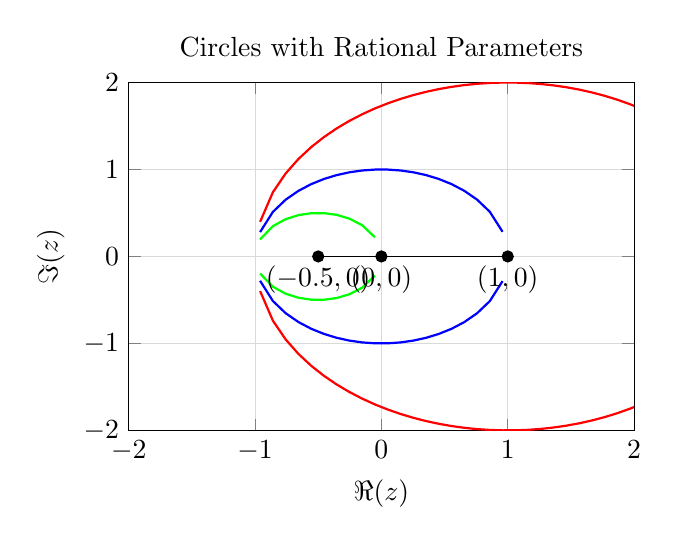
\begin{tikzpicture}
\begin{axis}[
    width=8cm,
    height=6cm,
    xlabel={$\Re(z)$},
    ylabel={$\Im(z)$},
    title={Circles with Rational Parameters},
    xmin=-2, xmax=2,
    ymin=-2, ymax=2,
    grid=major,
    grid style={gray!30},
    samples=100
]

% Draw circles with rational parameters
\addplot[blue, thick] {sqrt(1-x^2)};
\addplot[blue, thick] {-sqrt(1-x^2)};
\addplot[red, thick] {sqrt(4-(x-1)^2)};
\addplot[red, thick] {-sqrt(4-(x-1)^2)};
\addplot[green, thick] {sqrt(0.25-(x+0.5)^2)};
\addplot[green, thick] {-sqrt(0.25-(x+0.5)^2)};

% Mark centers
\addplot[black, mark=*, mark size=2pt] coordinates {(0,0) (1,0) (-0.5,0)};
\node[below] at (axis cs:0,0) {$(0,0)$};
\node[below] at (axis cs:1,0) {$(1,0)$};
\node[below] at (axis cs:-0.5,0) {$(-0.5,0)$};

\end{axis}
\end{tikzpicture}
\caption{Examples of circles with rational centers and radii. Each circle is determined by three rational numbers (center coordinates and radius), making the set countable as it injects into $\mathbb{Q}^3$.}
\end{figure}

% Visualization for disjoint intervals
\begin{figure}[h]
\centering
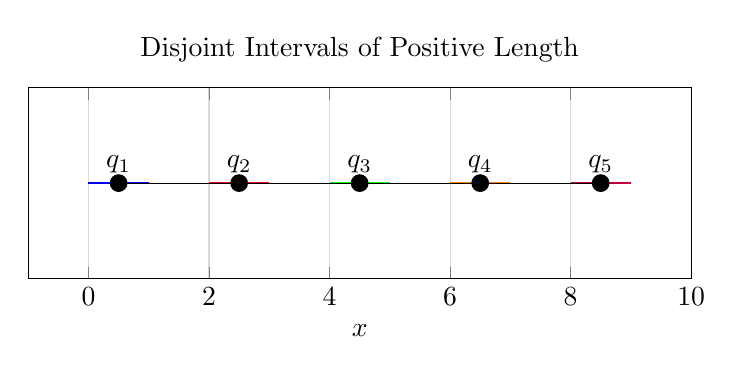
\begin{tikzpicture}
\begin{axis}[
    width=10cm,
    height=4cm,
    xlabel={$x$},
    ylabel={},
    title={Disjoint Intervals of Positive Length},
    xmin=-1, xmax=10,
    ymin=-0.5, ymax=0.5,
    grid=major,
    grid style={gray!30},
    samples=100,
    ytick=\empty
]

% Draw several disjoint intervals
\addplot[blue, thick] coordinates {(0,0) (1,0)};
\addplot[red, thick] coordinates {(2,0) (3,0)};
\addplot[green, thick] coordinates {(4,0) (5,0)};
\addplot[orange, thick] coordinates {(6,0) (7,0)};
\addplot[purple, thick] coordinates {(8,0) (9,0)};

% Mark rational points in each interval
\addplot[black, mark=*, mark size=3pt] coordinates {(0.5,0) (2.5,0) (4.5,0) (6.5,0) (8.5,0)};

% Add labels
\node[above] at (axis cs:0.5,0) {$q_1$};
\node[above] at (axis cs:2.5,0) {$q_2$};
\node[above] at (axis cs:4.5,0) {$q_3$};
\node[above] at (axis cs:6.5,0) {$q_4$};
\node[above] at (axis cs:8.5,0) {$q_5$};

\end{axis}
\end{tikzpicture}
\caption{Disjoint intervals of positive length. Each interval contains a rational number, and since the intervals are disjoint, these rationals are distinct, creating an injection into $\mathbb{Q}$.}
\end{figure}

\bigskip\noindent\textbf{Solution:}  
(a) Each circle is determined by a rational radius and two rational coordinates → set is countable.  
(b) Each disjoint interval must contain a distinct rational number → inject into \( \mathbb{Q} \), which is countable.\qed



\begin{problembox}[2.20: Countable Support for Real Function]
Let \( f \) be a real-valued function on \( [0,1] \). Suppose there exists \( M > 0 \) such that for any finite set of points \( \{x_1, \dots, x_n\} \subset [0,1] \),  
\[
|f(x_1)| + \dots + |f(x_n)| \le M
\]  
Let \( S = \{x \in [0,1] \mid f(x) \ne 0\} \). Prove that \( S \) is countable.
\end{problembox}

\noindent\textbf{Strategy:} Partition $S$ into sets $S_k = \{x : |f(x)| > 1/k\}$ for each positive integer $k$. Show that each $S_k$ is finite by using the bounded sum condition. Then $S$ is a countable union of finite sets, hence countable.

% Visualization of function with countable support
\begin{figure}[h]
\centering
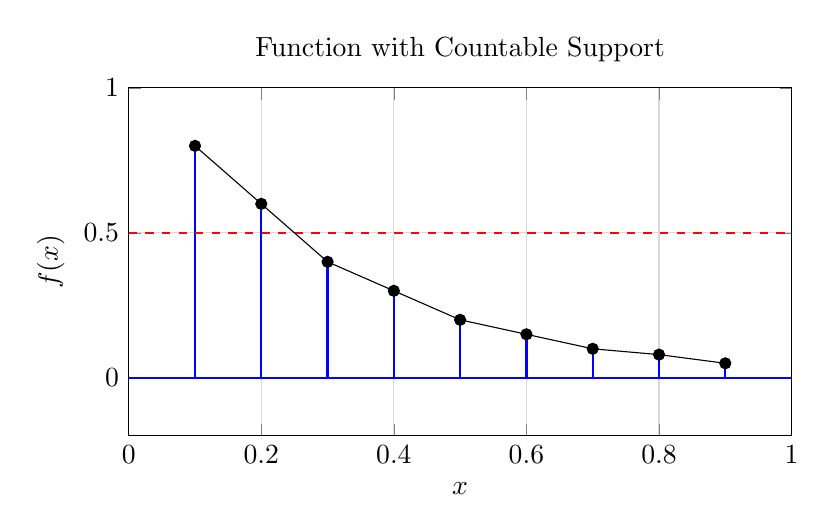
\begin{tikzpicture}
\begin{axis}[
    width=10cm,
    height=6cm,
    xlabel={$x$},
    ylabel={$f(x)$},
    title={Function with Countable Support},
    xmin=0, xmax=1,
    ymin=-0.2, ymax=1,
    grid=major,
    grid style={gray!30}
]

% Draw function with countable support
\addplot[blue, thick] coordinates {(0,0) (0.1,0) (0.1,0.8) (0.1,0) (0.2,0) (0.2,0.6) (0.2,0) (0.3,0) (0.3,0.4) (0.3,0) (0.4,0) (0.4,0.3) (0.4,0) (0.5,0) (0.5,0.2) (0.5,0) (0.6,0) (0.6,0.15) (0.6,0) (0.7,0) (0.7,0.1) (0.7,0) (0.8,0) (0.8,0.08) (0.8,0) (0.9,0) (0.9,0.05) (0.9,0) (1,0)};

% Add horizontal line for bound
\addplot[red, dashed, thick] coordinates {(0,0.5) (1,0.5)};
\node[right] at (axis cs:1,0.5) {$M = 0.5$};

% Mark support points
\addplot[black, mark=*, mark size=2pt] coordinates {(0.1,0.8) (0.2,0.6) (0.3,0.4) (0.4,0.3) (0.5,0.2) (0.6,0.15) (0.7,0.1) (0.8,0.08) (0.9,0.05)};

\end{axis}
\end{tikzpicture}
\caption{A function with countable support. The function is zero except at countably many points. The support $S = \{x : f(x) \neq 0\}$ is countable because each set $S_k = \{x : |f(x)| > 1/k\}$ is finite due to the bounded sum condition.}
\end{figure}

\bigskip\noindent\textbf{Solution:}  
Let $S = \{x \in [0,1] \mid f(x) \ne 0\}$. We want to prove that $S$ is countable.
An element $x$ is in $S$ if and only if $|f(x)| > 0$.
This is equivalent to saying that for each $x \in S$, there exists a positive integer $k$ such that $|f(x)| > 1/k$.

Let's define a collection of sets based on this idea. For each positive integer $k$, let:
\[ S_k = \left\{ x \in [0,1] \mid |f(x)| > \frac{1}{k} \right\} \]
The set $S$ is the union of all such sets:
\[ S = \bigcup_{k=1}^{\infty} S_k \]
If we can prove that each set $S_k$ is finite, then $S$ will be a countable union of finite sets, which is itself a countable set.

Let's consider a specific set $S_k$. Let $\{x_1, x_2, \dots, x_n\}$ be any finite collection of distinct points in $S_k$.
By the definition of $S_k$, we have $|f(x_i)| > 1/k$ for each $i=1, \dots, n$.
If we sum these values, we get:
\[ |f(x_1)| + |f(x_2)| + \dots + |f(x_n)| > \frac{1}{k} + \frac{1}{k} + \dots + \frac{1}{k} = \frac{n}{k} \]
The problem states that for any finite set of points, this sum is bounded by $M$:
\[ |f(x_1)| + |f(x_2)| + \dots + |f(x_n)| \le M \]
Combining these inequalities, we get:
\[ \frac{n}{k} < \sum_{i=1}^n |f(x_i)| \le M \implies \frac{n}{k} \le M \implies n \le kM \]
This result means that any finite subset of $S_k$ can have at most $kM$ elements. This implies that the set $S_k$ itself must be finite and contain at most $\lfloor kM \rfloor$ elements.

Since each $S_k$ is a finite set, their union $S = \bigcup_{k=1}^{\infty} S_k$ is a countable union of finite sets. Therefore, $S$ is a countable set.\qed



\begin{problembox}[2.21: Fallacy in Countability of Intervals]
Find the fallacy in the following "proof" that the set of all intervals of positive length is countable:  
Let \( \{x_1, x_2, \ldots\} \) be the rationals. Every interval contains a rational \( x_n \) with minimal index \( n \).  
Assign to the interval the smallest such \( n \). This gives a function from intervals to \( \mathbb{N} \), so the set of intervals is countable.
\end{problembox}

\noindent\textbf{Strategy:} Identify that the function is not injective. Many different intervals may contain the same rational with minimal index, so this does not establish a one-to-one correspondence between intervals and natural numbers.

\bigskip\noindent\textbf{Solution:}  
The function \( F \) is not injective — many intervals may have the same smallest-index rational.  
So this does not establish a one-to-one correspondence between intervals and \( \mathbb{N} \).  
Hence, the proof is invalid.\qed

\section{Additive Set Functions}

\subsection*{Definitions and Theorems}

\begin{definition}[Additive Function]
A function $f: \mathcal{P}(S) \to \mathbb{R}$ is additive if $f(A \cup B) = f(A) + f(B)$ whenever $A \cap B = \emptyset$.
\end{definition}

\begin{theorem}[Properties of Additive Functions]
For an additive function $f: \mathcal{P}(S) \to \mathbb{R}$ and any sets $A, B \subseteq S$:
\begin{enumerate}
\item $f(A \cup B) = f(A) + f(B - A)$
\item $f(A \cup B) = f(A) + f(B) - f(A \cap B)$
\end{enumerate}
\end{theorem}

\begin{theorem}[Inclusion-Exclusion Principle]
For an additive function $f$ and any sets $A_1, A_2, \ldots, A_n$:
\begin{align*}
f\left(\bigcup_{i=1}^n A_i\right) &= \sum_{i=1}^n f(A_i) - \sum_{1 \leq i < j \leq n} f(A_i \cap A_j) \\
&\quad + \sum_{1 \leq i < j < k \leq n} f(A_i \cap A_j \cap A_k) - \cdots + (-1)^{n+1} f\left(\bigcap_{i=1}^n A_i\right)
\end{align*}
\end{theorem}



\begin{problembox}[2.22: Additive Set Functions]
Let \( S \) be the collection of all subsets of a given set \( T \).  
A function \( f: S \to \mathbb{R} \) is additive if:
\[
f(A \cup B) = f(A) + f(B)
\quad \text{whenever } A \cap B = \emptyset
\]  
Prove:  
\[
f(A \cup B) = f(A) + f(B - A), \quad 
f(A \cup B) = f(A) + f(B) - f(A \cap B)
\]
\end{problembox}

\noindent\textbf{Strategy:} For the first identity, write $A \cup B$ as a disjoint union $A \cup (B-A)$ and apply the additivity property. For the second identity, decompose $A$ and $B$ into disjoint pieces using set differences and intersections, then use additivity and solve for the desired expression.

\bigskip\noindent\textbf{Solution:}  
Let $f: S \to \mathbb{R}$ be an additive function, meaning $f(X \cup Y) = f(X) + f(Y)$ whenever $X \cap Y = \emptyset$.

\textbf{Part 1:} Prove $f(A \cup B) = f(A) + f(B - A)$.
We can write the set $A \cup B$ as a disjoint union: $A \cup B = A \cup (B - A)$. The sets $A$ and $B-A$ (the part of $B$ not in $A$) are disjoint by definition.
Using the additivity property on this disjoint union:
\[ f(A \cup B) = f(A \cup (B-A)) = f(A) + f(B-A) \]
This proves the first identity.

\textbf{Part 2:} Prove $f(A \cup B) = f(A) + f(B) - f(A \cap B)$.
We start by decomposing $A$ and $B$ into disjoint pieces.
The set $A$ can be written as the disjoint union $A = (A - B) \cup (A \cap B)$. By additivity:
\[ f(A) = f(A - B) + f(A \cap B) \implies f(A-B) = f(A) - f(A \cap B) \]
The set $B$ can be written as the disjoint union $B = (B - A) \cup (A \cap B)$. By additivity:
\[ f(B) = f(B - A) + f(A \cap B) \implies f(B-A) = f(B) - f(A \cap B) \]
Now, we write $A \cup B$ as a union of three pairwise disjoint sets:
\[ A \cup B = (A - B) \cup (B - A) \cup (A \cap B) \]
Using the additivity property:
\[ f(A \cup B) = f(A-B) + f(B-A) + f(A \cap B) \]
Substitute the expressions we found for $f(A-B)$ and $f(B-A)$:
\begin{align*}
f(A \cup B) &= \big(f(A) - f(A \cap B)\big) + \big(f(B) - f(A \cap B)\big) + f(A \cap B) \\
&= f(A) + f(B) - f(A \cap B) - f(A \cap B) + f(A \cap B) \\
&= f(A) + f(B) - f(A \cap B)
\end{align*}
This proves the second identity.\qed



\begin{problembox}[2.23: Solving for Total Measure from Functional Equations]

Refer to Exercise 2.22. Assume \(f\) is additive and assume also that the following relations hold for two particular subsets \(A\) and \(B\) of \(T\):
\[
f(A \cup B) = f(A') + f(B') - f(A')f(B')
\]
\[
f(A \cap B) = f(A)f(B), \quad f(A) + f(B) \ne f(T),
\]
where \(A' = T - A, B' = T - B\). Prove that these relations determine \(f(T)\), and compute the value of \(f(T)\).
\end{problembox}

\noindent\textbf{Strategy:} Use the additivity property to express $f(A')$ and $f(B')$ in terms of $f(T)$, $f(A)$, and $f(B)$. Substitute these expressions into the first given equation. Then use the standard inclusion-exclusion formula for $f(A \cup B)$ and the second given relation to set up a quadratic equation in $f(T)$. Solve this equation and use the third condition to determine the unique solution.

\bigskip\noindent\textbf{Solution:}

We are given that the function \(f\) is additive, meaning \(f(X \cup Y) = f(X) + f(Y)\) for any disjoint sets \(X\) and \(Y\). For any subset \(X \subseteq T\), its complement \(X' = T - X\) is disjoint from \(X\) and their union is \(T\). The additive property therefore implies \(f(T) = f(X) + f(X')\), which gives us:
\begin{itemize}
\item \(f(A') = f(T) - f(A)\)
\item \(f(B') = f(T) - f(B)\)
\end{itemize}
We substitute these into the first given relation:
\begin{align*}
f(A \cup B) =& \big(f(T) - f(A)\big) + \big(f(T) - f(B)\big) \\
&- \big(f(T) - f(A)\big)\big(f(T) - f(B)\big) \\
=& 2f(T) - f(A) - f(B)  \\
&- \left[ f(T)^2 - f(T)f(A) - f(T)f(B) + f(A)f(B) \right] \\
=& 2f(T) - f(A) - f(B) - f(T)^2 \\
&+ f(T)f(A) + f(T)f(B) - f(A)f(B)
\end{align*}
Next, we use the standard inclusion-exclusion principle for an additive function, which states \(f(A \cup B) = f(A) + f(B) - f(A \cap B)\). From the second given relation, we know \(f(A \cap B) = f(A)f(B)\). Substituting this gives:
\[
f(A \cup B) = f(A) + f(B) - f(A)f(B)
\]
Now we set the two expressions for \(f(A \cup B)\) equal to each other:
\begin{align*}
&f(A) + f(B) - f(A)f(B) \\
=& 2f(T) - f(A) - f(B) - f(T)^2 + f(T)f(A) + f(T)f(B) - f(A)f(B)
\end{align*}
The \( -f(A)f(B) \) terms on each side cancel. We move all remaining terms to one side to form a quadratic equation in terms of \(f(T)\):
\[
f(T)^2 - 2f(T) - f(T)f(A) - f(T)f(B) + 2f(A) + 2f(B) = 0
\]
Factoring out \(f(T)\) and constant terms:
\[
f(T)^2 - f(T)\big(2 + f(A) + f(B)\big) + 2\big(f(A) + f(B)\big) = 0
\]
This quadratic equation can be factored as:
\[
\big(f(T) - 2\big) \big(f(T) - [f(A) + f(B)]\big) = 0
\]
This implies two possible solutions for \(f(T)\):
\begin{enumerate}
\item \(f(T) = 2\)
\item \(f(T) = f(A) + f(B)\)
\end{enumerate}
Finally, we use the third given relation, \(f(A) + f(B) \ne f(T)\), to eliminate the second possibility.
Therefore, the relations uniquely determine the value of \(f(T)\). That value is 2.
\[
\boxed{f(T) = 2}
\]\qed

\section{Solving and Proving Techniques}

\subsection*{Proving Set Equality}
\begin{itemize}
\item Use element-chasing: assume $x \in$ one side and show $x \in$ the other side, then reverse
\item Use set-theoretic identities and properties of union, intersection, and set difference
\item Break down complex sets into simpler components using distributive laws
\item Consider cases when dealing with piecewise definitions or different scenarios
\end{itemize}

\subsection*{Proving Function Properties}
\begin{itemize}
\item For injectivity: assume $f(x_1) = f(x_2)$ and show $x_1 = x_2$
\item For surjectivity: given any $y$ in codomain, find an $x$ in domain such that $f(x) = y$
\item For bijectivity: prove both injectivity and surjectivity
\item Use the definition of function composition: $(g \circ f)(x) = g(f(x))$
\item For piecewise functions, determine which piece applies based on the input value
\end{itemize}

\subsection*{Proving Relation Properties}
\begin{itemize}
\item For reflexivity: check if $(x,x) \in R$ for all $x$ in the set
\item For symmetry: check if $(x,y) \in R$ implies $(y,x) \in R$
\item For transitivity: check if $(x,y), (y,z) \in R$ implies $(x,z) \in R$
\item Use specific counterexamples to disprove properties
\item Consider edge cases and special values when testing properties
\end{itemize}

\subsection*{Proving Countability}
\begin{itemize}
\item Show a bijection exists with $\mathbb{N}$ or a known countable set
\item Use the fact that countable unions of countable sets are countable
\item Show the set injects into a known countable set
\item For finite sets, count the elements directly
\item Use the fact that removing a countable set from an uncountable set leaves an uncountable set
\end{itemize}

\subsection*{Proving Uncountability}
\begin{itemize}
\item Use Cantor's diagonal argument to show no bijection exists with $\mathbb{N}$
\item Show the set has strictly greater cardinality than a known uncountable set
\item Use the fact that power sets have strictly greater cardinality than the original set
\item Construct a contradiction by assuming countability and finding an element not in any enumeration
\end{itemize}

\subsection*{Working with Additive Functions}
\begin{itemize}
\item Use the definition: $f(A \cup B) = f(A) + f(B)$ when $A \cap B = \emptyset$
\item Decompose sets into disjoint unions to apply additivity
\item Use inclusion-exclusion principle for overlapping sets
\item Express complements in terms of the universal set: $f(A') = f(T) - f(A)$
\item Set up equations using known relationships and solve for unknown values
\end{itemize}

\subsection*{Proving Equivalence of Conditions}
\begin{enumerate}
\item Show each condition implies the next one in the chain
\item Show the last condition implies the first one (completing the cycle)
\item Use the fact that if $A \Rightarrow B$ and $B \Rightarrow A$, then $A \iff B$
\item Use contrapositive when direct implication is difficult
\item Break complex conditions into simpler logical components
\end{enumerate}

\subsection*{Constructing Bijections}
\begin{enumerate}
\item Identify the domain and codomain clearly
\item Define the function rule explicitly
\item Prove injectivity by showing $f(x_1) = f(x_2) \Rightarrow x_1 = x_2$
\item Prove surjectivity by showing every element in codomain has a preimage
\item Use piecewise definitions when different rules apply to different parts of the domain
\end{enumerate}

\subsection*{Working with Images and Preimages}
\begin{itemize}
\item Use definitions: $f(A) = \{f(x) : x \in A\}$ and $f^{-1}(Y) = \{x : f(x) \in Y\}$
\item Remember that $f(A \cap B) \subseteq f(A) \cap f(B)$ with equality only for injective functions
\item Use the fact that $f(A \cup B) = f(A) \cup f(B)$ always holds
\item For inverse images, use $f^{-1}(Y_1 \cup Y_2) = f^{-1}(Y_1) \cup f^{-1}(Y_2)$
\item Remember that $f[f^{-1}(Y)] = Y$ if and only if $f$ is surjective
\end{itemize}